\documentclass[10pt,twocolumn]{article}
\usepackage[margin=0.7in]{geometry}
\usepackage[utf8]{inputenc}
\usepackage[T1]{fontenc}
\usepackage{lmodern}
\usepackage{graphicx}
\usepackage{booktabs}
\usepackage{amsmath}
\usepackage{hyperref}
\usepackage{enumitem}
\usepackage{float}
\usepackage{pgfplotstable}

\graphicspath{{../outputs/figures/}{outputs/figures/}{figures/}}
\newcommand{\tablepath}{}
\IfFileExists{model_metrics.csv}{}{%
    \IfFileExists{../outputs/tables/model_metrics.csv}{%
        \renewcommand{\tablepath}{../outputs/tables/}
    }{%
        \IfFileExists{outputs/tables/model_metrics.csv}{%
            \renewcommand{\tablepath}{outputs/tables/}
        }{%
            \renewcommand{\tablepath}{tables/}
        }%
    }%
}
\newcommand{\csvpath}[1]{\tablepath#1}

\pgfplotstableset{
lemontable/.style={
    col sep=comma,
    every head row/.style={before row=\toprule, after row=\midrule},
    every last row/.style={after row=\bottomrule}
}
}

\pgfplotstableread[col sep=comma]{\csvpath{model_metrics.csv}}\metricstable
\pgfplotstableread[col sep=comma]{\csvpath{interaction_regression_key_terms.csv}}\regressiontable

\newcommand{\tabnum}[4]{%
    \pgfplotstablegetelem{#1}{#2}\of#3%
    \pgfmathprintnumber[fixed,precision=#4]{\pgfplotsretval}%
}

\title{Can Words Mitigate the Market for Lemons?\\Text Mining Evidence from Spanish Used-Car Listings}
\author{Josep Serra-Riera}
\date{}

\begin{document}
\maketitle

\begin{abstract}
This project studies whether listing text mitigates information asymmetry in the Spanish used-car market. Using 180{,}514 online car listings collected from \textit{milanuncios.com}, I build a text-based disclosure index that captures informative maintenance signals, transparency cues, honest defect disclosure, and promotional language. The empirical strategy combines a hedonic price model with text-mining techniques grounded in the course material: text normalization, dictionary-based feature extraction, TF-IDF n-grams, and supervised residual modeling. The analysis compares a structured baseline model that uses only observable characteristics with models augmented by textual information. Text improves predictive accuracy beyond structured variables: the holdout $R^2$ rises from 0.839 in the baseline to 0.845 with disclosure features and 0.852 with TF-IDF residual text. In the interaction regression, a one-standard-deviation increase in the disclosure index is associated with an estimated 2.1\% higher price, conditional on observables. Private sellers disclose less on average and receive lower prices, but the marginal return to disclosure is not statistically different from that of professionals. The project contributes an interpretable way to operationalize the classic ``lemons'' problem in a contemporary online market, linking microeconomic theory on adverse selection with practical natural language processing tools.
\end{abstract}

\section{Introduction}
Used-car markets are a canonical setting for adverse selection because sellers typically know more about vehicle quality than buyers. Akerlof's lemons framework predicts that when quality is hard to observe, high-quality sellers may not receive a fair price and market performance deteriorates. Online platforms partially change this environment because sellers provide free-form textual descriptions in addition to structured fields such as price, mileage, and year. These texts may either reduce information asymmetry through credible disclosure or worsen it through vague promotional language.

This paper studies whether more informative listing text is associated with higher prices in Spanish used-car ads. The central hypothesis is that disclosure-rich language works as a trust signal. I expected this effect to be stronger for private sellers, who lack dealership reputation and formal screening mechanisms. Rather than treating text mining as a standalone prediction task, the project uses NLP to answer a microeconomic question about market transparency.

The project focuses on Spain for two reasons. First, the used-car market is economically important because vehicles are durable goods with heterogeneous quality, so information frictions are likely to matter for both buyers and sellers. Second, the dataset contains naturally occurring listing language rather than survey responses or laboratory choices, which makes it possible to study how economic signals are actually expressed in marketplace text. This gives the project a practical contribution: it shows how simple text-mining tools can help translate an abstract microeconomic concept into an observable variable.

\section{Background}
Akerlof (1970) formalized the lemons problem as a consequence of asymmetric information between buyers and sellers. Subsequent work has shown that online platforms can attenuate these frictions by expanding information disclosure, search, and reputation. In car markets, disclosure is particularly relevant because maintenance history, accident information, and ownership details are costly for buyers to verify ex ante.

From an NLP perspective, the project is close to document representation and supervised learning tasks. Term-weighting schemes such as TF-IDF and linear predictive models are well suited to sparse, high-dimensional ad text. At the same time, a dictionary-based disclosure index offers interpretability, allowing the project to tie specific linguistic signals back to economic theory.

The most closely related economic idea is that disclosure can act as a signal when direct verification is difficult. Lewis (2011), in the context of eBay Motors, shows that online disclosure is economically meaningful and affects market outcomes. My project is more modest, but it follows the same intuition: when sellers voluntarily reveal concrete information, buyers may update beliefs about product quality and seller credibility. This is especially relevant in a decentralized market where not all sellers have the same reputation or legal guarantees.

There are also two complementary NLP motivations behind the empirical design. The first is interpretability: a small disclosure lexicon makes it possible to explain why a listing receives a high or low score, which is useful in a short academic report. The second is predictive validation: if text still improves price prediction after controlling for year, mileage, power, seller type, and region, then textual information is likely capturing some economically relevant variation rather than simple noise.

\section{Methodology}
The raw data are cleaned to parse prices, mileage, registration year, horsepower, seller type, and region. Listing text is built from the ad title and description, normalized to address encoding noise, lowercased, accent-stripped, and tokenized through regular-expression preprocessing.

The key explanatory variable is a disclosure index. It increases with mentions of maintenance and transparency cues such as \textit{revisiones al d\'{\i}a}, \textit{garant\'{\i}a}, \textit{km reales}, or \textit{facturas}; it also rewards defect disclosure and numeric detail, while penalizing purely promotional language such as \textit{oportunidad} or \textit{como nuevo}. The score is standardized to produce a z-score.

Three empirical models are estimated. First, a structured hedonic model predicts log price from mileage, age, power, seller type, and region. Second, the structured model is augmented with disclosure features. Third, a TF-IDF residual model predicts the part of price left unexplained by observables, isolating the value of textual information. Finally, an interaction regression tests whether disclosure matters more for private sellers.

The use of log price is standard in hedonic settings because it reduces skewness and makes coefficients easier to interpret in percentage terms. The baseline model therefore asks a simple question: how much of price can be explained by observable characteristics alone? The second model adds text-derived disclosure variables to test whether an interpretable summary of listing language improves on that benchmark. The third model goes one step further by vectorizing the full text with TF-IDF unigrams and bigrams, then predicting the residual from the baseline model. This design is useful because it separates the information contained in text from the information already captured by structured fields.

The methodology intentionally balances simplicity and economic meaning. More complex language models could likely extract additional signals, but the objective here is not to maximize raw predictive performance at any cost. Instead, the goal is to show that even relatively simple text representations can operationalize a concept from microeconomic theory. In that sense, the disclosure index functions as the central bridge between NLP and the economics question.

\section{Experimentation}
The project uses the public \textit{spanish\_used\_car\_market} dataset from Zenodo. After cleaning, implausible or malformed observations are removed, keeping 180{,}514 listings with realistic values for price, mileage, year, horsepower, and seller type. The average listing price is 11{,}708 euros, median price is 8{,}900 euros, mean mileage is roughly 133{,}539 km, and private sellers represent 27.3\% of the cleaned sample. Performance is evaluated on a holdout split using RMSE, MAE, and $R^2$ for log price.

The pipeline is fully reproducible from one command: \texttt{python project.py}. The code produces tables and figures in the \texttt{outputs/} directory.

For the predictive exercises, I sample up to 60{,}000 listings and split them into training and test sets using a fixed random seed. The structured and disclosure-augmented models are estimated with ridge regression, which is convenient because it remains stable when many dummy variables are created from seller type, brand, and region. For the text residual model, the descriptions are converted into TF-IDF features with Spanish stopwords removed, unigrams and bigrams retained, and a maximum vocabulary size of 15{,}000 features. The final residual model is then estimated with elastic-net regularization.

Table~\ref{tab:desc} summarizes the cleaned sample. The difference between mean and median prices already suggests substantial heterogeneity in the market, which is exactly the type of environment where asymmetric information can be important. The fact that private sellers make up only around a quarter of listings also matters for interpretation, because the market is not dominated by a single seller type.

\begin{table}[H]
\centering
\caption{Descriptive statistics}
\label{tab:desc}
\resizebox{\columnwidth}{!}{%
\pgfplotstabletypeset[
lemontable,
columns={n_listings,mean_price_eur,median_price_eur,mean_km,mean_vehicle_age,private_share},
columns/n_listings/.style={column name=Listings, column type=r, fixed, precision=0},
columns/mean_price_eur/.style={column name=Mean price, column type=r, fixed, precision=0},
columns/median_price_eur/.style={column name=Median price, column type=r, fixed, precision=0},
columns/mean_km/.style={column name=Mean km, column type=r, fixed, precision=0},
columns/mean_vehicle_age/.style={column name=Mean age, column type=r, fixed, precision=1},
columns/private_share/.style={column name=Private share, column type=r, fixed, precision=3}
]{\csvpath{descriptive_stats.csv}}
}
\end{table}

\section{Results and Analysis}
Table~\ref{tab:metrics} reports the predictive comparison across models, while Table~\ref{tab:reg} isolates the disclosure effect in the interaction regression. The baseline hedonic model already performs well, with a holdout $R^2$ of 0.839. Adding the disclosure lexicon improves this to 0.845 and lowers RMSE from 0.397 to 0.390. The strongest performance comes from the TF-IDF residual model, which reaches an $R^2$ of 0.852 and RMSE of 0.381. This confirms that textual descriptions contain information not captured by mileage, age, horsepower, seller type, region, and brand alone.

\begin{table}[H]
\centering
\caption{Predictive performance}
\label{tab:metrics}
\resizebox{\columnwidth}{!}{%
\begin{tabular}{lrrr}
\toprule
Model & RMSE & MAE & $R^2$ \\
\midrule
Structured baseline
& \tabnum{0}{rmse_log_price}{\metricstable}{4}
& \tabnum{0}{mae_log_price}{\metricstable}{4}
& \tabnum{0}{r2}{\metricstable}{4} \\
Structured + disclosure lexicon
& \tabnum{1}{rmse_log_price}{\metricstable}{4}
& \tabnum{1}{mae_log_price}{\metricstable}{4}
& \tabnum{1}{r2}{\metricstable}{4} \\
Structured + TF-IDF residual text
& \tabnum{2}{rmse_log_price}{\metricstable}{4}
& \tabnum{2}{mae_log_price}{\metricstable}{4}
& \tabnum{2}{r2}{\metricstable}{4} \\
\bottomrule
\end{tabular}
}
\end{table}

\begin{table}[H]
\centering
\caption{Key interaction-regression terms}
\label{tab:reg}
\resizebox{\columnwidth}{!}{%
\begin{tabular}{lrrr}
\toprule
Term & Coefficient & Std. error & $p$-value \\
\midrule
Intercept
& \tabnum{0}{coefficient}{\regressiontable}{4}
& \tabnum{0}{std_error}{\regressiontable}{4}
& \tabnum{0}{p_value}{\regressiontable}{4} \\
Disclosure index
& \tabnum{1}{coefficient}{\regressiontable}{4}
& \tabnum{1}{std_error}{\regressiontable}{4}
& \tabnum{1}{p_value}{\regressiontable}{4} \\
Private seller
& \tabnum{2}{coefficient}{\regressiontable}{4}
& \tabnum{2}{std_error}{\regressiontable}{4}
& \tabnum{2}{p_value}{\regressiontable}{4} \\
Disclosure index $\times$ private seller
& \tabnum{3}{coefficient}{\regressiontable}{4}
& \tabnum{3}{std_error}{\regressiontable}{4}
& \tabnum{3}{p_value}{\regressiontable}{4} \\
\bottomrule
\end{tabular}
}
\end{table}

\begin{figure}[H]
\centering
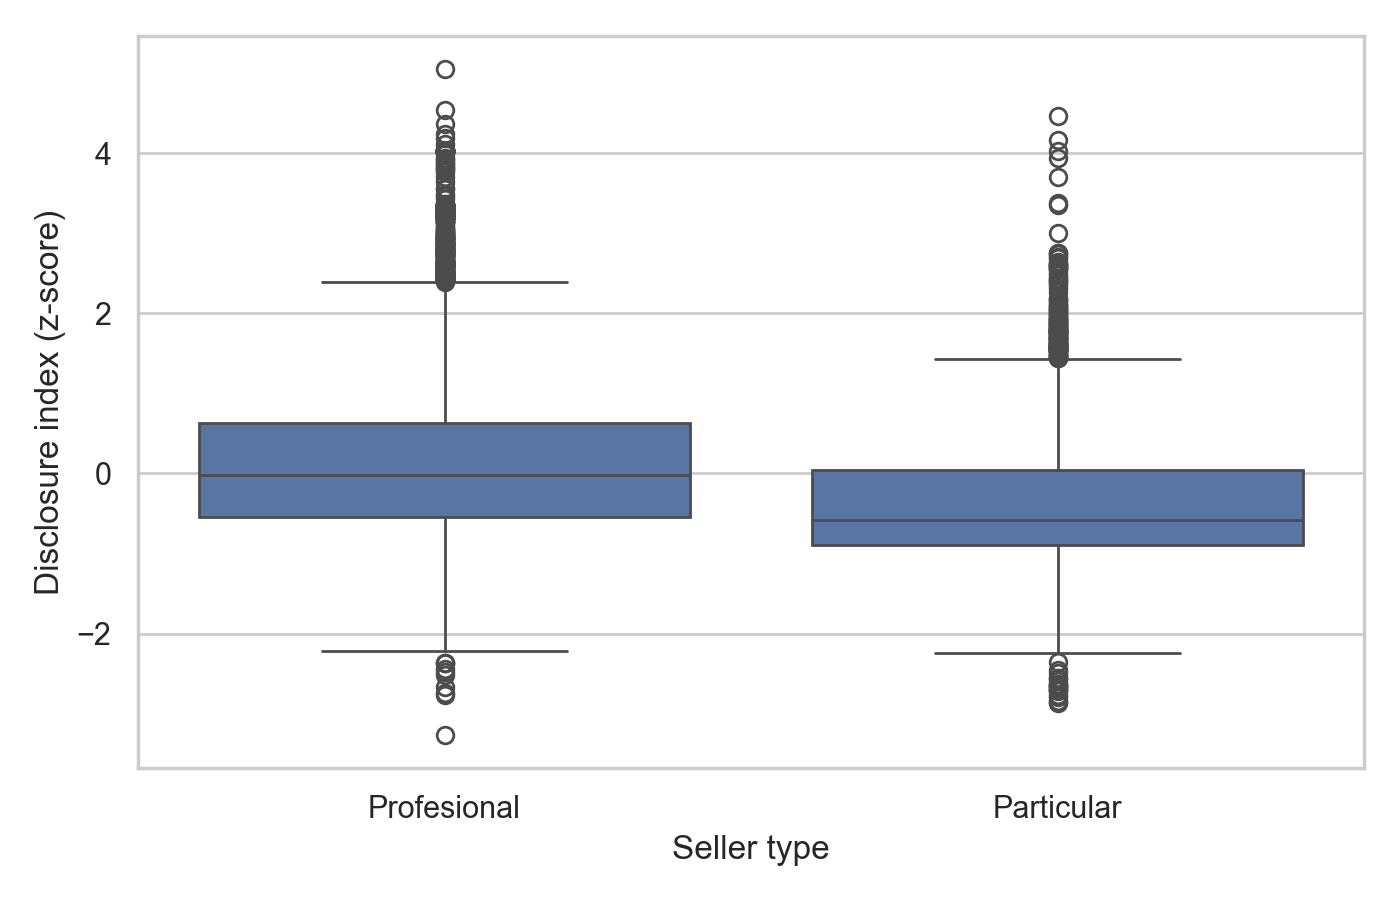
\includegraphics[width=\columnwidth]{disclosure_by_seller.png}
\caption{Disclosure index by seller type}
\end{figure}

\begin{figure}[H]
\centering
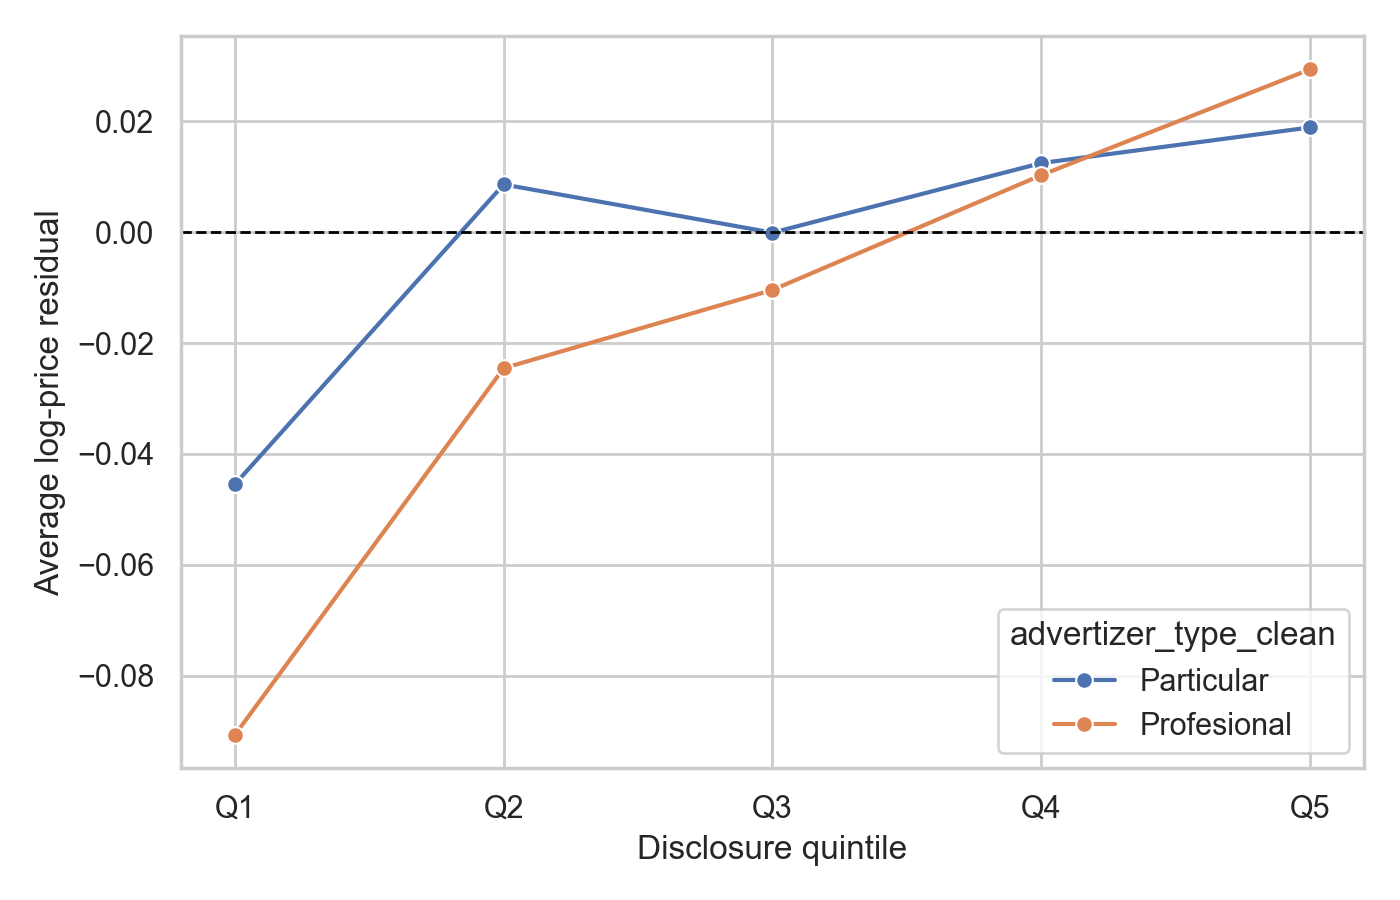
\includegraphics[width=\columnwidth]{residuals_by_disclosure_quintile.png}
\caption{Average baseline residual by disclosure quintile}
\end{figure}

\begin{figure}[H]
\centering
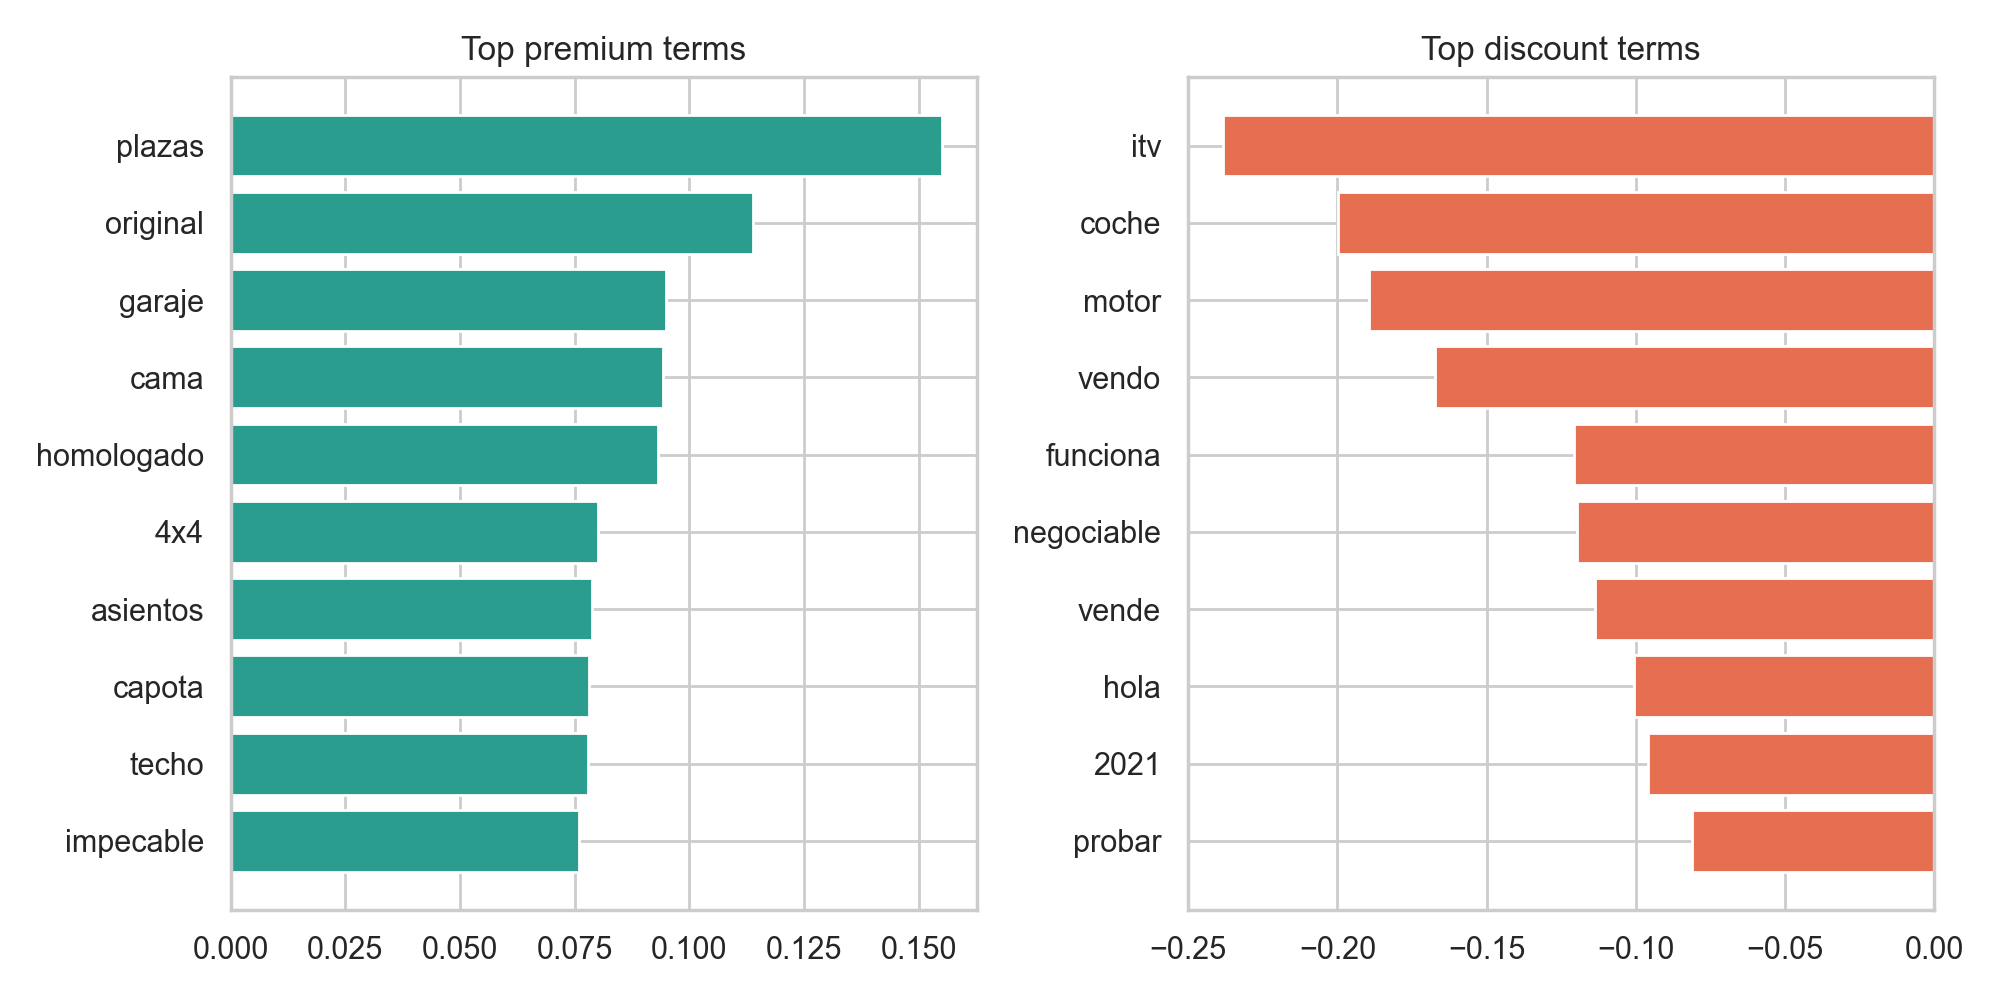
\includegraphics[width=\columnwidth]{top_price_terms.png}
\caption{Top TF-IDF terms associated with price residuals}
\end{figure}

The disclosure regression also supports the information story. The coefficient on the standardized disclosure index is 0.0211 and highly significant, which implies that a one-standard-deviation increase in disclosure is associated with approximately 2.1\% higher price, conditional on observables. Private sellers face an estimated 6.7\% price discount relative to professionals, again conditional on controls. However, the disclosure interaction for private sellers is statistically insignificant. This means that the data support a positive role for disclosure overall, but not a distinctly larger marginal return for private sellers.

The descriptive evidence suggests an interesting interpretation. Figure 1 shows that professional sellers have a higher average disclosure index than private sellers. This likely reflects the institutionalized language of dealerships, which often mention warranty, documentation, or included transfer services in templated descriptions. The TF-IDF model reinforces the pattern: premium-associated terms include \textit{garant\'{\i}a}, \textit{revisiones}, \textit{nacional}, and \textit{homologado}, while discount-associated terms include \textit{negociable}, \textit{vendo}, \textit{funciona}, and \textit{itv}. These terms are economically meaningful because they distinguish richer, verification-oriented descriptions from language that is either generic or associated with lower-quality vehicles.

The size of the predictive improvements is also informative. The jump from the baseline to the disclosure model is not huge, but it is systematic across the main error metrics. This is a plausible pattern in an application like used cars, where structured attributes already explain much of the price, yet text still adds marginal information. Put differently, the results do not imply that text dominates mechanical characteristics such as age or mileage; rather, they show that language contains incremental information once those variables are already controlled for.

At the same time, the regression results should not be interpreted as pure causal effects. More informative language may be correlated with unobserved seller professionalism, vehicle condition, or marketing effort. That limitation is important, but it does not undermine the main contribution of the project. Even under a predictive and correlational interpretation, the evidence is still consistent with the idea that informative language reduces uncertainty in a lemons-type market. For the purposes of this assignment, that is the key empirical insight.

\section{Conclusions}
This project connects a classic microeconomic problem to modern text-mining methods. By treating free-form listing language as a source of information disclosure, the analysis shows how online texts can be converted into interpretable economic signals. The framework is intentionally simple and replicable, relying on TF-IDF features, linear models, and a theory-driven disclosure dictionary.

The main substantive conclusion is that words matter: textual information improves price prediction and higher disclosure is associated with higher prices. At the same time, the null interaction for private sellers suggests that disclosure is not enough to fully close the trust gap between seller types. Future work could extend the project in three directions: incorporating richer Spanish language models, collecting full descriptions rather than previews, and linking price outcomes to realized sale duration or dealer reputation. Even in its current form, the project provides evidence that online language can partially mitigate the informational frictions at the heart of the lemons problem.

More broadly, the project illustrates why text mining can be useful in economics beyond sentiment analysis. In many applied settings, the relevant information is not only numerical but also embedded in descriptions, complaints, contracts, advertisements, or reviews. A simple workflow based on text cleaning, interpretable features, and standard predictive models can therefore provide a bridge between economic theory and messy real-world data. That is the main lesson I would emphasize from this project.

\section{Bibliography}
\begin{itemize}[leftmargin=*]
    \item Akerlof, G. A. (1970). The market for ``lemons'': Quality uncertainty and the market mechanism. \textit{Quarterly Journal of Economics}, 84(3), 488--500.
    \item Campillo S\'anchez, P., \& Uceda Mart\'inez, P. (2020). \textit{spanish\_used\_car\_market: Coches de segunda mano a la venta en Espa\~na}. Zenodo. \url{https://doi.org/10.5281/zenodo.4252636}
    \item Lewis, G. (2011). Asymmetric information, adverse selection and online disclosure: The case of eBay Motors. \textit{American Economic Review}, 101(4), 1535--1546.
\end{itemize}

\end{document}
